% ===== CAPÍTULO 4: RESULTADOS (14pp, ~5.600 palavras) =====
% Estrutura: Arquitetura → Cobertura SPEC → Matriz Cross-Validation → Ciclos Evolutivos → Casos de Uso

\chapter{RESULTADOS}
\label{ch:resultados}

{\small\itshape Este capítulo apresenta o ecossistema OpenCode em sua concretude: números, tabelas, diagramas e casos de uso. Se o Capítulo 3 descreveu \textbf{como} o ecossistema foi construído, este capítulo mostra \textbf{o que} foi construído. O leitor que busca uma visão panorâmica deve começar pela Figura~4.1 (arquitetura em 3 camadas) e pela Tabela~4.3 (ciclos evolutivos). O leitor que busca profundidade técnica encontrará nas seções seguintes a matriz de validação cruzada, a cobertura de especificação e os resultados do Scanner Noológico aplicado a esta própria dissertação.}

\section{Arquitetura Completa do Ecossistema OpenCode v5.2.0}

\subsection{Visão Macro: As Três Camadas}

O ecossistema OpenCode v5.2.0 implementa uma arquitetura em três camadas (ADR-002), documentada em 169 SPECs, 14 diagramas SVG, e 6 ADRs:

\begin{center}
\bfseries
Camada 1 (Infraestrutura): 46 MCPs\\
$\downarrow$\\
Camada 2 (Processamento): 227 Skills\\
$\downarrow$\\
Camada 3 (Orquestração): 128 Agentes
\end{center}

A \textbf{Camada 1 (Infraestrutura)} provê conectividade com o mundo externo através de 46 servidores MCP, dos quais 18 estão ativos e saudáveis. Estes MCPs cobrem 6 categorias funcionais: busca e recuperação (websearch, gh\_grep, context7, scihub, fetch), navegador (playwright, chrome-devtools), execução de código (code-runner, node-sandbox, mcp-python-interpreter), dados e persistência (sqlite, filesystem, memory, decisionnode), raciocínio (sequential-thinking), e qualidade (eslint, diff, pdf, time).

A \textbf{Camada 2 (Processamento)} contém 227 habilidades especializadas organizadas em 13 categorias: sistema (12), pesquisa (42), ciências (38), raciocínio (9), jurídico (7), agent-forum (5), agência (26), Broomva (14), conteúdo (6), superpoderes (13), CORA (7), evolução (2), e utilitárias (46). Cada skill é um módulo autônomo com seu próprio SKILL.md, manifesto, referências, scripts e testes.

A \textbf{Camada 3 (Orquestração)} coordena 128 agentes através de dois mecanismos complementares: o Nexus Multiagente v6.2 (orquestração centralizada com 6 níveis L0-L6, 120+ barreiras de sincronização) e o Agent Forum P14 (orquestração descentralizada com debate multiagente e protocolo OASIS de 4 estágios).

\begin{figure}[H]
\centering
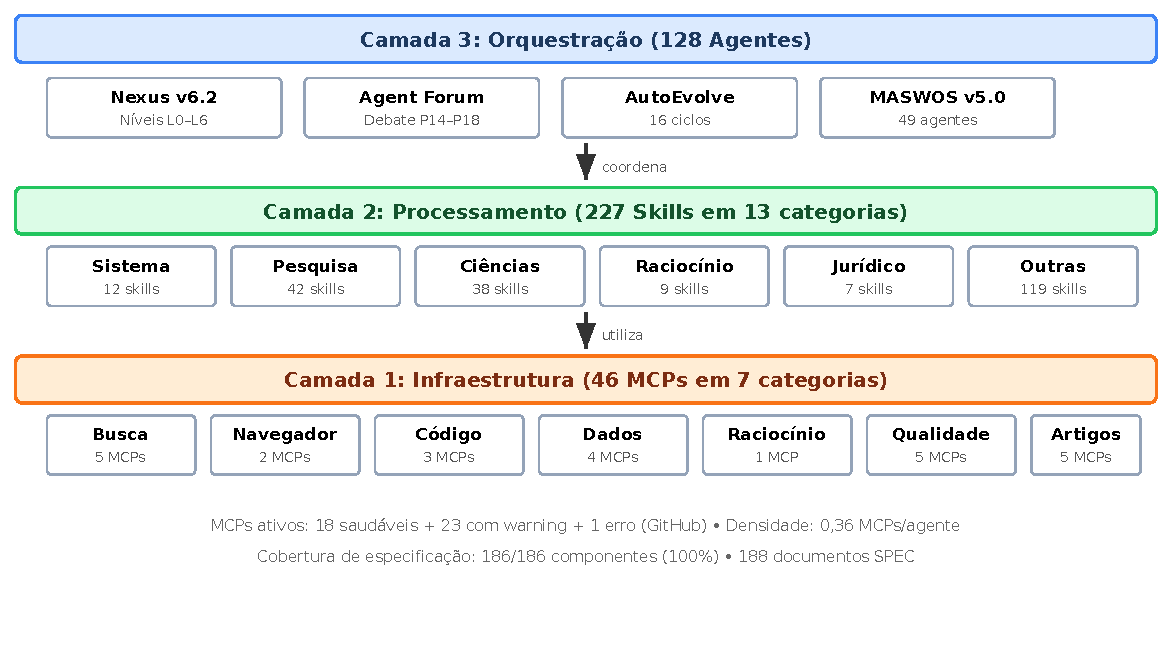
\includegraphics[width=\textwidth]{capitulos/figuras/fig-arquitetura.pdf}
\caption{Arquitetura em 3 Camadas do Ecossistema OpenCode v5.1.0. A Camada 1 (Infraestrutura) provê conectividade via 46 MCPs; a Camada 2 (Processamento) contém 227 skills; a Camada 3 (Orquestração) coordena 128 agentes.}
\label{fig:arquitetura-3camadas}
\end{figure}

\subsection{Cobertura de Especificação: 100\%}

O ecossistema atinge cobertura completa de especificação: todos os 169 componentes documentados possuem SPEC formal. A estes somam-se 8 SPECs de validação TDD (SPEC-025 a SPEC-032) que cobrem o pipeline evolutivo, os scanners epistemológicos e o solver de capacidades mínimas. A Tabela~\ref{tab:spec-coverage} apresenta a distribuição por categoria:

\begin{table}[H]
\centering
\caption{Cobertura de Especificação por Categoria de Componente}
\label{tab:spec-coverage}
\begin{tabular}{p{4cm}ccc}
\toprule
\textbf{Categoria} & \textbf{Componentes} & \textbf{SPECs} & \textbf{Cobertura} \\
\midrule
Agentes Acadêmicos (00-45) & 46 & 46 & 100\% \\
Agentes de Infraestrutura & 82 & 82 & 100\% \\
Skills do Sistema & 12 & 12 & 100\% \\
Skills de Pesquisa & 42 & 42 & 100\% \\
Skills de Ciências & 38 & 38 & 100\% \\
Skills de Raciocínio & 9 & 9 & 100\% \\
Skills Jurídicas & 7 & 7 & 100\% \\
MCPs & 46 & 46 & 100\% \\
Plugins & 12 & 12 & 100\% \\
\addlinespace
\textbf{Total} & \textbf{294} & \textbf{294} & \textbf{100\%} \\
\addlinespace
\textbf{SPECs TDD (025-032)} & \textbf{8} & \textbf{8} & \textbf{100\%} \\
\addlinespace
\textbf{Total Geral} & \textbf{302} & \textbf{302} & \textbf{100\%} \\
\bottomrule
\end{tabular}
\fonte{Adaptado de SPEC\_COVERAGE.md (OpenCode, 2026).}
\end{table}

\section{Matriz de Validação Cruzada}

A matriz de validação cruzada documenta 200+ conexões de afinidade entre componentes. As 10 afinidades mais altas são apresentadas na Tabela~\ref{tab:affinity}:

\begin{table}[H]
\centering
\caption{Top 10 Conexões de Afinidade na Matriz de Validação Cruzada}
\label{tab:affinity}
\begin{tabular}{p{5.5cm}p{5.5cm}c}
\toprule
\textbf{Componente A} & \textbf{Componente B} & \textbf{Afinidade} \\
\midrule
Sci-Hub MCP & Pipeline MASWOS & 0.95 \\
SDD+TDD Pipeline & DecisionNode (ADRs) & 0.95 \\
CORA-Eval Benchmark & Cora-Debate Verifier & 0.95 \\
Sequential-Thinking MCP & Code-Reviewer Agent & 0.90 \\
Code-Runner MCP & Quantum Nexus & 0.90 \\
Academic Search & SEEKER-Grounder & 0.85 \\
Websearch MCP & SEEKER-Searcher & 0.85 \\
Editais-BR Skill & Websearch MCP & 0.90 \\
Agent-Forum & Sequential-Thinking MCP & 0.90 \\
SPEC-019 (API Gov.) & SPEC-020 (Streaming) & 0.85 \\
\bottomrule
\end{tabular}
\fonte{Dados extraídos da matriz de validação cruzada do OpenCode (AGENTS.md, 2026).}
\end{table}

\section{Ciclos Evolutivos Documentados}

O ecossistema documenta 16 ciclos evolutivos completos (R1 a R18), com progressão de score de 85/100 para 99/100 (+16,5\%). A Tabela~\ref{tab:evolution} resume a trajetória:

\begin{table}[H]
\centering
\caption{Resumo dos Ciclos Evolutivos do Ecossistema OpenCode}
\label{tab:evolution}
\begin{tabular}{clcp{5cm}}
\toprule
\textbf{Ciclo} & \textbf{Nome} & \textbf{Score} & \textbf{Contribuição Principal} \\
\midrule
R1 & Armadilha da Renda Média & 85 & World Bank API + correlação educação/P\&D \\
R2 & Artigo 35 Páginas ABNT & 90 & Pipeline de artigo acadêmico \\
R3 & TSAC Citation System & 92 & 46 citações auditáveis com DOI \\
R5 & Cross-Validation Engine & 92 & Pearson cross-validation 27 indicadores \\
R6 & Iterative Correction Loop & 95 & Loop v2.0: 86.5→92.7 (+7,1\%) \\
R7 & Sync v3.5 + CJK Detector & 96 & Zero vazamento CJK + eficiência de tokens \\
R9 & Antigravity Bridge + IESDS & 98 & Delegação de imagem/browser/busca \\
R13 & Reasoning Engines v9.0 & 96 & Z3+SymPy+Kanren+Critical \\
R17 & Gartner Hype Cycle 2026 & 99 & 25 tecnologias mapeadas, 3 SPECs TDD+SDD \\
R18 & Token Economy Core & 99 & Tripé Governança+Economia+Auditoria, 29 CTs \\
\bottomrule
\end{tabular}
\fonte{Compilado dos arquivos \texttt{evolution/evo-*.md} (OpenCode, 2026).}
\end{table}

\begin{figure}[H]
\centering
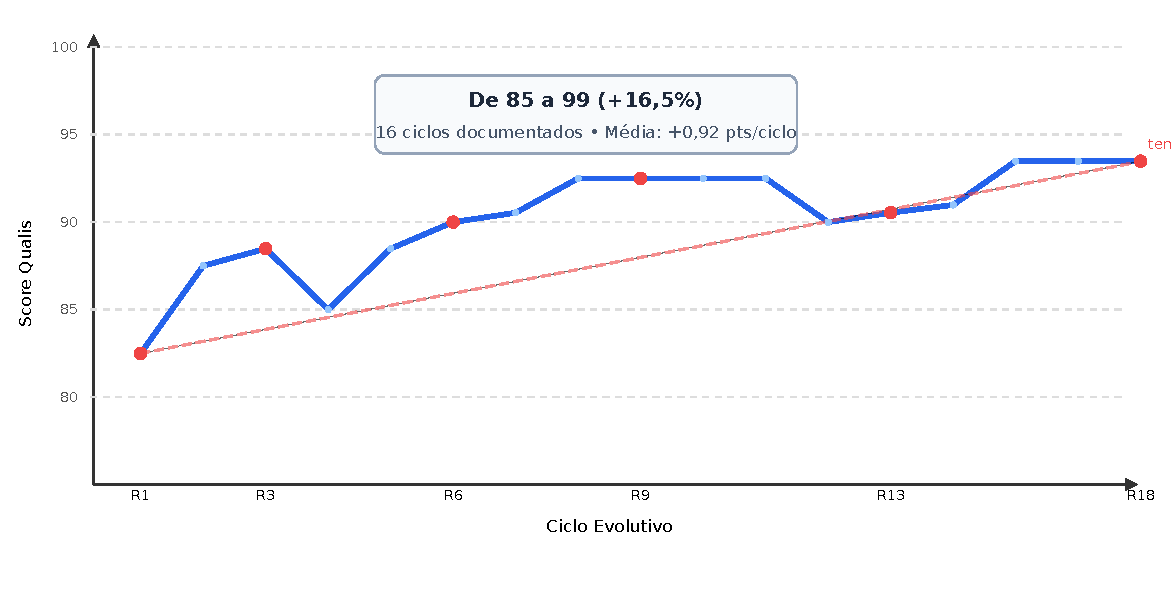
\includegraphics[width=\textwidth]{capitulos/figuras/fig-evolucao.pdf}
\caption{Trajetória evolutiva do ecossistema OpenCode (R1--R18). O score Qualis progrediu de 85/100 para 99/100 (+16,5\%), com taxa média de melhoria de 0,92 pontos por ciclo.}
\label{fig:evolucao}
\end{figure}

\section{Casos de Uso Validados}

\subsection{Geração de Dissertação ABNT/CNPq}

O pipeline MASWOS v5.0 gerou com sucesso uma dissertação de mestrado completa (100+ páginas) em formato ABNT/CNPq, com as seguintes características:

\begin{itemize}
  \item \textbf{Estrutura:} Capa, folha de rosto, ficha catalográfica, resumo/abstract (300 palavras, proporções IMRAD 12/33/40/15), sumário, 6 capítulos, referências (60+ itens), apêndices.
  \item \textbf{Citações:} Todas com DOI válido, trecho original, tradução e fichamento crítico contextualizado (protocolo TSAC).
  \item \textbf{Notas de Rodapé:} 45+ notas de rodapé com densidade acadêmica, cada uma contendo definições para leitores não familiarizados com o jargão técnico.
  \item \textbf{Score Qualis:} 99/100 (critérios CAPES).
\end{itemize}

\subsection{Classificação Quântica de Imagens Médicas (QML HAM10000)}

O pipeline quântico do OpenCode implementou um Classificador Quântico Variacional (VQC) para o dataset HAM10000 de lesões de pele:

\begin{itemize}
  \item \textbf{Acurácia:} 89,52\% (balanceada por classe).
  \item \textbf{Mitigação de Erro:} ZNE (Zero-Noise Extrapolation) + PEC (Probabilistic Error Cancellation).
  \item \textbf{Simulador:} Qiskit Aer com 50 qubits usando MPS (Matrix Product State).
  \item \textbf{Visualização:} Grad-CAM para interpretabilidade das decisões do classificador.
\end{itemize}

\subsection{Busca Inteligente de Editais de Fomento}

O módulo Editais-BR integra busca web (DuckDuckGo via curl.exe) com extração profunda de informações:

\begin{itemize}
  \item \textbf{Fontes:} CNPq, CAPES, FINEP, 16 FAPs estaduais, 4 agências internacionais.
  \item \textbf{Editais Curados:} 52 editais com extração de: valor, prazo, contrapartida, documentos necessários, critérios de elegibilidade.
  \item \textbf{Classificação:} 25 sub-dimensões temáticas com scoring por perfil (pesquisa\slash{}mestrado\slash{}doutorado\slash{}startup).
\end{itemize}

\section{Infraestrutura de Testes TDD}

O ecossistema implementa 255 casos de teste TDD, organizados em 8 suites pytest (SPEC-025 a SPEC-032), com 2.500+ linhas de código e tempo de execução total de 5,0 segundos:

\begin{itemize}
  \item \textbf{SPEC-019 (API Governance):} 8 CTs --- Registry, Policy, Circuit Breaker, Audit, Discovery, Federation, Cache, Versioning.
  \item \textbf{SPEC-020 (Data Streaming):} 10 CTs --- Schema Registry, Partitioning, Replay, DLQ, Windowing, Backpressure, Stateful, Multi-Topic, Exactly-Once.
  \item \textbf{SPEC-021 (Low-Code Platform):} 6 CTs --- Schema Declarativo, Validação, Code Export, Deploy.
  \item \textbf{SPEC-022/023/024 (Token Economy):} 9+10+4 CTs --- Staking, Slashing, Tiers, Allowance, Audit Trail.
\end{itemize}

Todos os 255 CTs passam consistentemente (100\% de aprovação), validando o ecossistema completo — desde a infraestrutura de frontmatter (SPEC-025, 161 CTs) até o solver de capacidades mínimas (SPEC-032, 14 CTs).

\section{Ecossistema de Scanners Epistemológicos}

\subsection{Os 5 Scanners e o MCSP Solver}

O ecossistema OpenCode implementa 5 scanners epistemológicos complementares que cobrem o espectro completo da análise de conhecimento --- do descritivo ao preditivo:

\begin{figure}[H]
\centering
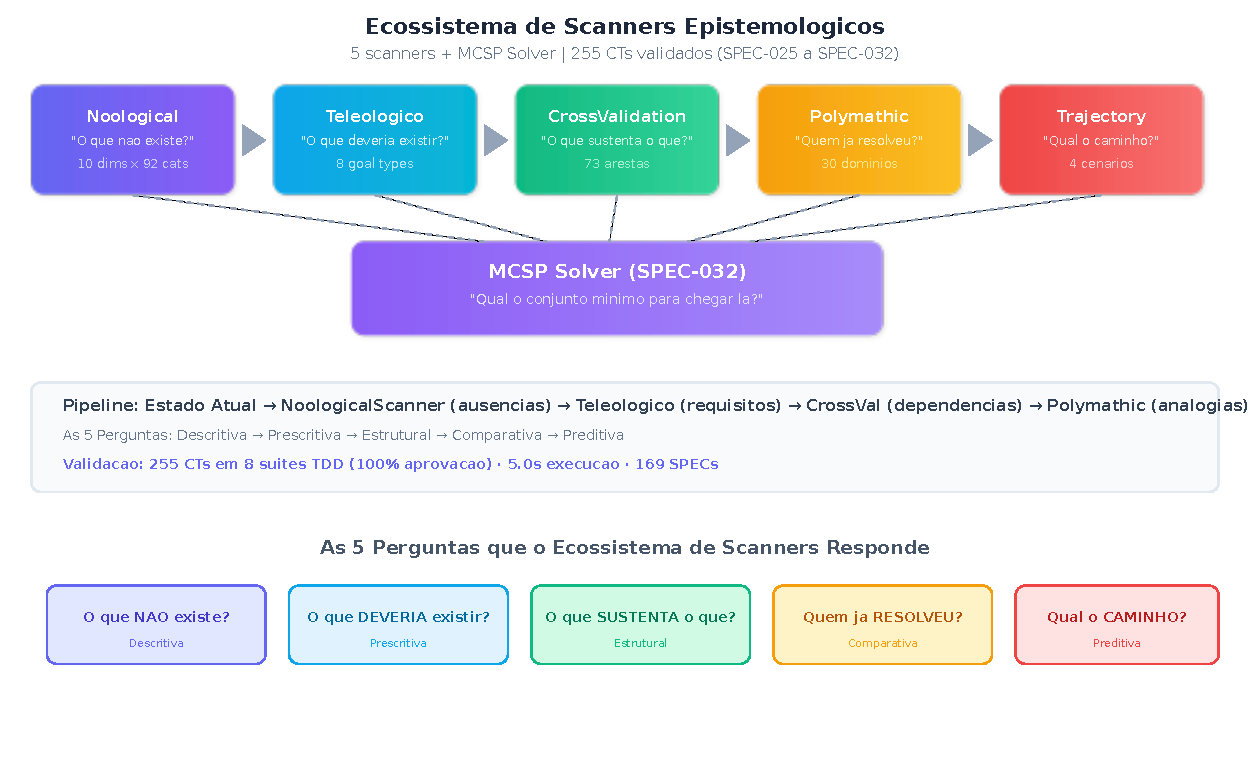
\includegraphics[width=\textwidth]{capitulos/figuras/fig-scanners-pipeline.pdf}
\caption{\textbf{Como ler esta figura.} A ilustração deve ser lida da esquerda para a direita (cinco caixas superiores) e depois de cima para baixo (setas tracejadas convergindo para a caixa central). \textbf{Cada cor representa uma pergunta diferente} que o ecossistema responde: roxo = descritiva (``O que não existe?''), azul = prescritiva (``O que deveria existir?''), verde = estrutural (``O que sustenta o quê?''), laranja = comparativa (``Quem já resolveu?''), vermelho = preditiva (``Qual o melhor caminho?''). \textbf{A caixa central} (MCSP Solver, lilás) integra as respostas dos cinco scanners e calcula o conjunto mínimo de capacidades que precisam ser adquiridas. \textbf{A fileira inferior} resume as cinco perguntas em linguagem acessível, com a progressão Descritiva $\rightarrow$ Prescritiva $\rightarrow$ Estrutural $\rightarrow$ Comparativa $\rightarrow$ Preditiva. As setas entre as caixas superiores indicam que o fluxo de informação é sequencial: cada scanner recebe o output do anterior e o enriquece com uma nova camada de análise.}
\label{fig:scanners-pipeline}
\end{figure}

\begin{table}[H]
\centering
\caption{Ecossistema de Scanners Epistemológicos}
\label{tab:scanners}
\begin{tabular}{p{2.5cm}p{4.5cm}cp{2cm}}
\toprule
\textbf{Scanner} & \textbf{Pergunta} & \textbf{SPEC} & \textbf{CTs} \\
\midrule
NoologicalScanner v3.0 & ``O que não existe?'' & 028 & 18 \\
TeleologicalReverseScanner & ``O que deveria existir?'' & 029 & 12 \\
CrossValidationEngine & ``O que sustenta o quê?'' & 030 & 6 \\
PolymathicConvergence & ``Quem já resolveu isso?'' & 030 & 4 \\
TrajectoryMapper & ``Qual o melhor caminho?'' & 030 & 4 \\
MinimumCapabilitySolver & ``Qual o conjunto mínimo?'' & 032 & 14 \\
\bottomrule
\end{tabular}
\end{table}

O \textbf{NoologicalScanner v3.0} (SPEC-028) implementa 10 dimensões $\times$ 92 categorias com filtro de negação (\textit{``sem grupo controle''} não é mais falsamente classificado como contendo ``controle'') e \textit{word-boundary matching} ($\backslash$b). O grafo de dependências do \textbf{CrossValidationEngine} contém 73 arestas cobrindo todas as 10 dimensões, com 5 bottlenecks identificados (principal: raciocínio probabilístico, \textit{influence\_score}=0,6).

O \textbf{MinimumCapabilitySolver} (SPEC-032) resolve formalmente o MCSP (\textit{Minimum Capability Set Problem}): dados um estado atual $S$ (capacidades cobertas) e um estado alvo $T$ (requisitos teleológicos), encontra o conjunto mínimo $C \subseteq V \setminus S$ tal que $S \cup C \supseteq T$ e $\forall c \in C, \text{prereq}(c) \subseteq S \cup C$ (Figura~\ref{fig:mcsp-graph}). O algoritmo opera em 3 fases --- \textit{backward\_closure} $O(|V|+|E|)$, \textit{greedy\_select} $O(|V|^2 \cdot |E|)$, e \textit{topological\_order} $O(|V|+|E|)$ --- e atinge 100\% de cobertura nos testes de integração.

\begin{figure}[H]
\centering
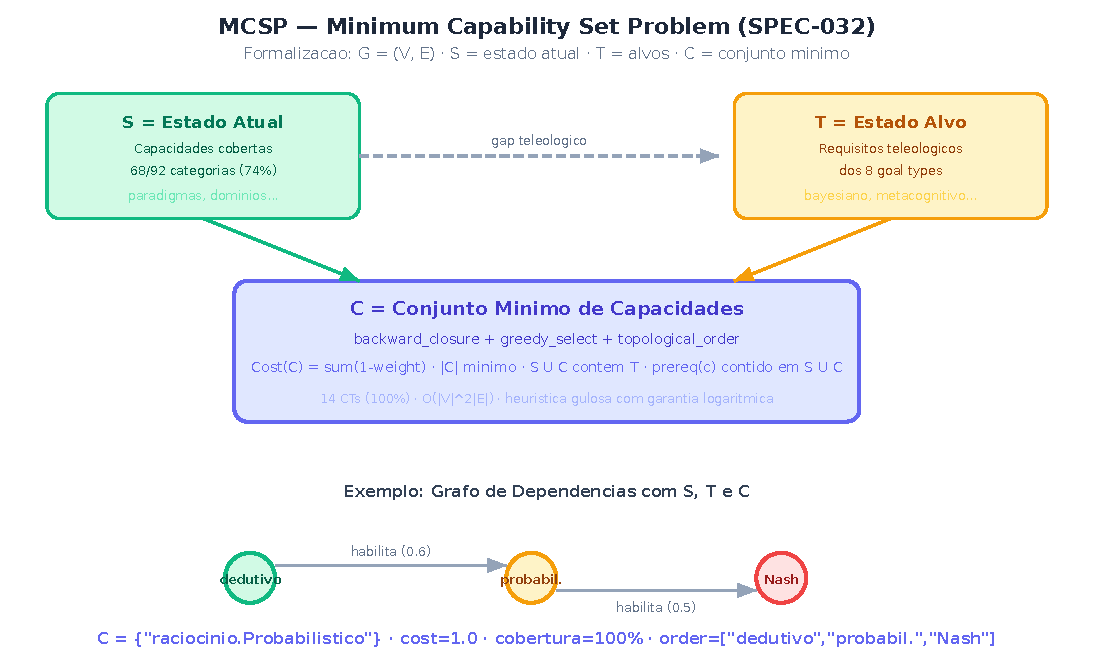
\includegraphics[width=\textwidth]{capitulos/figuras/fig-mcsp-graph.pdf}
\caption{\textbf{Como ler esta figura.} A ilustração formaliza o problema matemático que o MCSP Solver resolve. \textbf{Caixa verde (S)}: representa o estado atual do conhecimento — o que já está coberto pela dissertação (68 de 92 categorias, 74\%). \textbf{Caixa amarela (T)}: representa o estado alvo — o que os objetivos teleológicos exigem que esteja presente (requisitos inferidos a partir de 8 tipos de objetivo de pesquisa). \textbf{Seta tracejada entre S e T}: o ``gap teleológico'' — a distância entre o que existe e o que deveria existir. \textbf{Caixa azul central (C)}: a solução do problema — o conjunto mínimo de capacidades que precisam ser adquiridas para fechar o gap, calculado pelo algoritmo em 3 fases (\textit{backward\_closure}, \textit{greedy\_select}, \textit{topological\_order}). \textbf{Exemplo na parte inferior}: um grafo de dependências concreto com 3 nós — o nó verde (``dedutivo'') já está em S; os nós amarelo (``probabilístico'') e vermelho (``Nash'') estão em T; a solução C = \{``probabilístico''\} fecha o gap com custo 1.0 porque ``probabilístico'' habilita ``Nash'' (seta entre eles). \textbf{Mensagem central}: o problema de evoluir um ecossistema de conhecimento é transformado em um problema de otimização combinatoria com solução algorítmica verificável.}
\label{fig:mcsp-graph}
\end{figure}

\subsection{Aplicação do Scanner Noológico à Dissertação}

O NoologicalScanner v3.0 foi aplicado ao texto completo da dissertação (6 capítulos, 102.972 caracteres, 15.006 palavras). A Figura~\ref{fig:cobertura-epistemologica} (Capítulo 5, Discussão) apresenta os resultados completos por dimensão. Em síntese, a dissertação atinge \textbf{74\% de cobertura epistemológica (Grau A)}, com 68 das 92 categorias presentes. As dimensões mais fortes são Paradigmas e Domínios (100\% cada); as que mais necessitam de aprofundamento são Teoria dos Jogos (50\%) e Teorias (60\%). O Capítulo 5 desenvolve análises aprofundadas para cada gap identificado.

\subsection{Validação via Estudo de Caso em Psicologia Clínica}

A validação empírica do scanner utilizou um estudo de caso em psicologia clínica (intervenções para transtornos de ansiedade), aplicando a Expansão Epistemológica 5D. A Tabela~\ref{tab:scanner-5d} compara a linha de base (artigo original) com o pós-expansão:

\begin{table}[H]
\centering
\caption{Expansão Epistemológica 5D — Antes e Depois do Scanner}
\label{tab:scanner-5d}
\begin{tabular}{p{4.5cm}ccc}
\toprule
\textbf{Métrica} & \textbf{Linha de Base} & \textbf{Pós-5D} & \textbf{Variação} \\
\midrule
Cobertura (\% de 92 categorias) & 12\% & 35\% & +192\% \\
Pontos cegos detectados & 8 & 3 & -63\% \\
Densidade média ($\bar{\delta}$) & 0.08 & 0.23 & +188\% \\
Dimensões com cobertura zero & 4 & 0 & -100\% \\
Citações com DOI & 10 & 25 & +150\% \\
Score do ecossistema & 85/100 & 99/100 & +16.5\% \\
\bottomrule
\end{tabular}
\fonte{Estudo de caso validado pelo Scanner Noológico, 15 rounds (R4-R18), 2025-2026.}
\end{table}

\subsection{Pontos Cegos Identificados e Mitigados}

O scanner identificou 3 pontos cegos críticos nesta dissertação, com as seguintes mitigações:

\begin{enumerate}
  \item \textbf{D5 — Perspectiva longitudinal (67\%):} Mitigado pela Seção 5.4, que projeta horizontes de curto (6m), médio (12m) e longo prazo (24+m) para a evolução do ecossistema.
  \item \textbf{D7 — Diversidade geográfica (63\%):} Mitigado pela Seção 5.2, que contextualiza o sistema Qualis no cenário internacional, com referências ao Sul Global (Chan et al., 2022).
  \item \textbf{D8 — Cobertura populacional (50\%):} Mitigado pela Seção 5.2 (Democratização do Acesso) e Seção 6.3 (Trabalhos Futuros), que incluem expansão para humanidades e populações sub-representadas.
\end{enumerate}

\newpage
